\documentclass[preview]{standalone}

\usepackage{amsmath}
\usepackage{amssymb}
\usepackage{stellar}
\usepackage{bettelini}
\usepackage{wrapfig}
\usepackage{enumitem}

\hypersetup{
    colorlinks=true,
    linkcolor=black,
    urlcolor=blue,
    pdftitle={Stellar},
    pdfpagemode=FullScreen,
}

\begin{document}

\id{geoeconomica-commercio-mondiale}
\genpage

\section{Reti, nodi e flussi globali - il commercio mondiale}

\begin{snippet}{commercio-mondiale-alcuni-dati}
    \vspace*{-0.25cm}
    \begin{itemize}
        \item Le percentuali dei volumi del commercio per i diversi vettori di trasporto:
            \begin{itemize}
                \item Camion: 9\%
                \item Treno: 5\%
                \item Nave: 85\%
                \item Aereo: 1\%
            \end{itemize}
        \item Il commercio marittimo planetario si sviluppa nel XVIII\textdegree\, secolo;
        \item Nel XIX\textdegree\, secolo vengono costruiti i grandi canali navigabili di Suez e di
            Panama;
        \item Tra il 1950 e il 2017, il peso totale delle merci trasportate dal commercio mondiale
            è aumentato del 2000\%;
    \end{itemize} 
\end{snippet}

\subsection{Stretti e canali}

\begin{snippetdefinition}{stretto-definition}{Stretto}
    Uno \textit{stretto} è una zona d'acqua minima che collega due masse d'acqua.
\end{snippetdefinition}

\begin{snippetdefinition}{istmo-definition}{Istmo}
    Un \textit{istmo} è una zona di terra minima che collega due masse di terra.
\end{snippetdefinition}

\begin{snippet}{stretti-e-canali-famosi}
    %=== MAPPA ===
    \setlength{\intextsep}{0pt}%
    \begin{wrapfigure}{r}{.65\textwidth}
        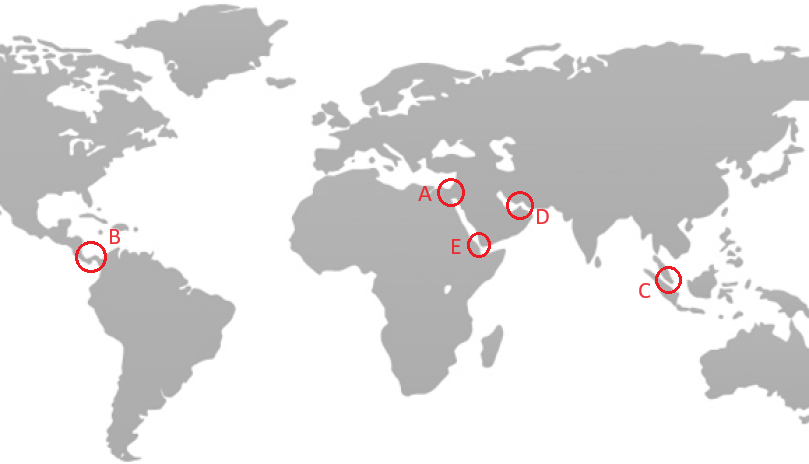
\includegraphics[width=.65\textwidth]{resources/mappa-stretti-canali.png}
        \vspace{-2.5cm}
    \end{wrapfigure}
    Le posizioni sulla cartina indicano:

    \begin{enumerate}[label=\Alph*:]
        \item Canale di Suez;
        \item Canale di Panama;
        \item Stretto di Malacca;
        \item Stretto di Ormuz;
        \item Bab el Mandeb.
    \end{enumerate}
    \wrapfill
\end{snippet}

\end{document}